% ******************************* PhD Thesis Template **************************
% Please have a look at the README.md file for info on how to use the template

\documentclass[a4paper,10pt,twoside,custommargin,times,numbered,print,index]{Classes/PhDThesisPSnPDF}

% ******************************************************************************
% ******************************* Class Options ********************************
% *********************** See README for more details **************************
% ******************************************************************************

% `a4paper'(The University of Cambridge PhD thesis guidelines recommends a page
% size a4 - default option) or `a5paper': A5 Paper size is also allowed as per
% the Cambridge University Engineering Deparment guidelines for PhD thesis
%
% `11pt' or `12pt'(default): Font Size 10pt is NOT recommended by the University
% guidelines
%
% `oneside' or `twoside'(default): Printing double side (twoside) or single
% side.
%
% `print': Use `print' for print version with appropriate margins and page
% layout. Leaving the options field blank will activate Online version.
%
% `index': For index at the end of the thesis
%
% `draftclassic': For draft mode without loading any images (same as draft in book)
%
% `draft': Special draft mode with line numbers, images, and water mark with
% timestamp and custom text. Position of the text can also be modified.
%
% `abstract': To generate only the title page and abstract page with
% dissertation title and name, to submit to the Student Registry
%
% `chapter`: This option enables only the specified chapter and it's references
%  Useful for review and corrections.
%
% ************************* Custom Page Margins ********************************
%
% `custommargin`: Use `custommargin' in options to activate custom page margins,
% which can be defined in the preamble.tex. Custom margin will override
% print/online margin setup.
%
% *********************** Choosing the Fonts in Class Options ******************
%
% `times' : Times font with math support. (The Cambridge University guidelines
% recommend using times)
%
% `fourier': Utopia Font with Fourier Math font (Font has to be installed)
%            It's a free font.
%
% `customfont': Use `customfont' option in the document class and load the
% package in the preamble.tex
%
% default or leave empty: `Latin Modern' font will be loaded.
%
% ********************** Choosing the Bibliography style ***********************
%
% `authoryear': For author-year citation eg., Krishna (2013)
%
% `numbered': (Default Option) For numbered and sorted citation e.g., [1,5,2]
%
% `custombib': Define your own bibliography style in the `preamble.tex' file.
%              `\RequirePackage[square, sort, numbers, authoryear]{natbib}'.
%              This can be also used to load biblatex instead of natbib
%              (See Preamble)
%
% **************************** Choosing the Page Style *************************
%
% `default (leave empty)': For Page Numbers in Header (Left Even, Right Odd) and
% Chapter Name in Header (Right Even) and Section Name (Left Odd). Blank Footer.
%
% `PageStyleI': Chapter Name next & Page Number on Even Side (Left Even).
% Section Name & Page Number in Header on Odd Side (Right Odd). Footer is empty.
%
% `PageStyleII': Chapter Name on Even Side (Left Even) in Header. Section Number
% and Section Name in Header on Odd Side (Right Odd). Page numbering in footer

% Uncomment to change page style
%\pagestyle{PageStyleII}

% ********************************** Preamble **********************************
% Preamble: Contains packages and user-defined commands and settings
% ******************************************************************************
% ****************************** Custom Margin *********************************

% Add `custommargin' in the document class options to use this section
% Set {innerside margin / outerside margin / topmargin / bottom margin}  and
% other page dimensions
\ifsetCustomMargin
  \RequirePackage[left=37mm,right=30mm,top=35mm,bottom=30mm]{geometry}
  \setFancyHdr % To apply fancy header after geometry package is loaded
\fi

% Add spaces between paragraphs
%\setlength{\parskip}{0.5em}
% Ragged bottom avoids extra whitespaces between paragraphs
\raggedbottom
% To remove the excess top spacing for enumeration, list and description
%\usepackage{enumitem}
%\setlist[enumerate,itemize,description]{topsep=0em}

% *****************************************************************************
% ******************* Fonts (like different typewriter fonts etc.)*************

% Add `customfont' in the document class option to use this section

\ifsetCustomFont
  % Set your custom font here and use `customfont' in options. Leave empty to
  % load computer modern font (default LaTeX font).
  %\RequirePackage{helvet}

  % For use with XeLaTeX
  %  \setmainfont[
  %    Path              = ./libertine/opentype/,
  %    Extension         = .otf,
  %    UprightFont = LinLibertine_R,
  %    BoldFont = LinLibertine_RZ, % Linux Libertine O Regular Semibold
  %    ItalicFont = LinLibertine_RI,
  %    BoldItalicFont = LinLibertine_RZI, % Linux Libertine O Regular Semibold Italic
  %  ]
  %  {libertine}
  %  % load font from system font
  %  \newfontfamily\libertinesystemfont{Linux Libertine O}
\fi

% *****************************************************************************
% **************************** Custom Packages ********************************

% ************************* Algorithms and Pseudocode **************************

%\usepackage{algpseudocode}
\usepackage{tikz}
\usepackage{pgfplots}
\usepgfplotslibrary{dateplot}
\pgfplotsset{compat=1.9}

\usepackage{inconsolata}

% Copyright 2017 Sergei Tikhomirov, MIT License
% https://github.com/s-tikhomirov/solidity-latex-highlighting/

\usepackage[final]{listings}
\usepackage{xcolor}

\definecolor{verylightgray}{rgb}{.97,.97,.97}

\lstdefinelanguage{Solidity}{
	keywords=[1]{anonymous, assembly, assert, balance, break, call, callcode, case, catch, class, constant, continue, contract, debugger, default, delegatecall, delete, do, else, emit, event, export, external, false, finally, for, function, gas, if, implements, import, in, indexed, instanceof, interface, internal, is, length, library, log0, log1, log2, log3, log4, memory, modifier, new, payable, pragma, private, protected, public, pure, push, require, return, returns, revert, selfdestruct, send, storage, struct, suicide, super, switch, then, this, throw, transfer, true, try, typeof, using, value, view, while, with, addmod, ecrecover, keccak256, mulmod, ripemd160, sha256, sha3}, % generic keywords including crypto operations
	keywordstyle=[1]\color{blue}\bfseries,
	keywords=[2]{address, bool, byte, bytes, bytes1, bytes2, bytes3, bytes4, bytes5, bytes6, bytes7, bytes8, bytes9, bytes10, bytes11, bytes12, bytes13, bytes14, bytes15, bytes16, bytes17, bytes18, bytes19, bytes20, bytes21, bytes22, bytes23, bytes24, bytes25, bytes26, bytes27, bytes28, bytes29, bytes30, bytes31, bytes32, enum, int, int8, int16, int24, int32, int40, int48, int56, int64, int72, int80, int88, int96, int104, int112, int120, int128, int136, int144, int152, int160, int168, int176, int184, int192, int200, int208, int216, int224, int232, int240, int248, int256, mapping, string, uint, uint8, uint16, uint24, uint32, uint40, uint48, uint56, uint64, uint72, uint80, uint88, uint96, uint104, uint112, uint120, uint128, uint136, uint144, uint152, uint160, uint168, uint176, uint184, uint192, uint200, uint208, uint216, uint224, uint232, uint240, uint248, uint256, var, void, ether, finney, szabo, wei, days, hours, minutes, seconds, weeks, years},	% types; money and time units
	keywordstyle=[2]\color{teal}\bfseries,
	keywords=[3]{block, blockhash, coinbase, difficulty, gaslimit, number, timestamp, msg, data, gas, sender, sig, value, now, tx, gasprice, origin},	% environment variables
	keywordstyle=[3]\color{violet}\bfseries,
	identifierstyle=\color{black},
	sensitive=false,
	comment=[l]{//},
	morecomment=[s]{/*}{*/},
	commentstyle=\color{gray}\ttfamily,
	stringstyle=\color{red}\ttfamily,
	morestring=[b]',
	morestring=[b]"
}

\lstset{
	language=Solidity,
	backgroundcolor=\color{white},
	extendedchars=true,
	basicstyle=\footnotesize\ttfamily,
	showstringspaces=false,
	showspaces=false,
	numbers=none,
	numberstyle=\footnotesize,
	numbersep=9pt,
	tabsize=2,
	breaklines=true,
	showtabs=false,
	captionpos=t
}


\usepackage[final]{listings}

\usepackage[a-3b]{pdfx}
 
%\usepackage{color}
%\definecolor{codecomment}{HTML}{808080}
%\definecolor{codekeyword}{HTML}{0039C1}
%\definecolor{codestring}{HTML}{397F39}
%\definecolor{bg}{HTML}{FFFFFF}
%\definecolor{codenumbers}{HTML}{999999}
%\lstdefinestyle{codestyle}{
%    backgroundcolor=\color{bg},
%    commentstyle=\color{codecomment},
%    keywordstyle=\color{codekeyword},
%    stringstyle=\color{codestring},
%    numberstyle=\tiny\color{codenumbers},
%    basicstyle=\ttfamily\footnotesize,
%    numbers=left,                    
%    numbersep=10pt,                  
%    showstringspaces=false,
%}
%
%\lstset{style=codestyle}


% ********************Captions and Hyperreferencing / URL **********************

% Captions: This makes captions of figures use a boldfaced small font.
%\RequirePackage[small,bf]{caption}

\RequirePackage[labelsep=space,tableposition=top]{caption}
\renewcommand{\figurename}{Fig.} %to support older versions of captions.sty


% *************************** Graphics and figures *****************************

%\usepackage{rotating}
%\usepackage{wrapfig}

% Uncomment the following two lines to force Latex to place the figure.
% Use [H] when including graphics. Note 'H' instead of 'h'
%\usepackage{float}
%\restylefloat{figure}

% Subcaption package is also available in the sty folder you can use that by
% uncommenting the following line
% This is for people stuck with older versions of texlive
%\usepackage{sty/caption/subcaption}
\usepackage{subcaption}

% ********************************** Tables ************************************
\usepackage{booktabs} % For professional looking tables
\usepackage{multirow}

%\usepackage{multicol}
%\usepackage{longtable}
%\usepackage{tabularx}


% *********************************** SI Units *********************************
\usepackage{siunitx} % use this package module for SI units


% ******************************* Line Spacing *********************************

% Choose linespacing as appropriate. Default is one-half line spacing as per the
% University guidelines

% \doublespacing
% \onehalfspacing
% \singlespacing


% ************************ Formatting / Footnote *******************************

% Don't break enumeration (etc.) across pages in an ugly manner (default 10000)
%\clubpenalty=500
%\widowpenalty=500

%\usepackage[perpage]{footmisc} %Range of footnote options


% *****************************************************************************
% *************************** Bibliography  and References ********************

%\usepackage{cleveref} %Referencing without need to explicitly state fig /table

% Add `custombib' in the document class option to use this section
\ifuseCustomBib
   \RequirePackage[square, sort, numbers, authoryear]{natbib} % CustomBib

% If you would like to use biblatex for your reference management, as opposed to the default `natbibpackage` pass the option `custombib` in the document class. Comment out the previous line to make sure you don't load the natbib package. Uncomment the following lines and specify the location of references.bib file

%\RequirePackage[backend=biber, style=numeric-comp, citestyle=numeric, sorting=nty, natbib=true]{biblatex}
%\addbibresource{References/references} %Location of references.bib only for biblatex, Do not omit the .bib extension from the filename.

\fi

% changes the default name `Bibliography` -> `References'
\renewcommand{\bibname}{References}


% ******************************************************************************
% ************************* User Defined Commands ******************************
% ******************************************************************************

% *********** To change the name of Table of Contents / LOF and LOT ************

%\renewcommand{\contentsname}{My Table of Contents}
%\renewcommand{\listfigurename}{My List of Figures}
%\renewcommand{\listtablename}{My List of Tables}
\newcommand{\code}[1]{\texttt{#1}}


% ********************** TOC depth and numbering depth *************************

\setcounter{secnumdepth}{2}
\setcounter{tocdepth}{2}


% ******************************* Nomenclature *********************************

% To change the name of the Nomenclature section, uncomment the following line

%\renewcommand{\nomname}{Symbols}


% ********************************* Appendix ***********************************

% The default value of both \appendixtocname and \appendixpagename is `Appendices'. These names can all be changed via:

%\renewcommand{\appendixtocname}{List of appendices}
%\renewcommand{\appendixname}{Appndx}

% *********************** Configure Draft Mode **********************************

% Uncomment to disable figures in `draft'
%\setkeys{Gin}{draft=true}  % set draft to false to enable figures in `draft'

% These options are active only during the draft mode
% Default text is "Draft"
%\SetDraftText{DRAFT}

% Default Watermark location is top. Location (top/bottom)
%\SetDraftWMPosition{bottom}

% Draft Version - default is v1.0
\SetDraftVersion{v4}

% Draft Text grayscale value (should be between 0-black and 1-white)
% Default value is 0.75
%\SetDraftGrayScale{0.8}


% ******************************** Todo Notes **********************************
%% Uncomment the following lines to have todonotes.

%\ifsetDraft
%	\usepackage[colorinlistoftodos]{todonotes}
%	\newcommand{\mynote}[1]{\todo[author=Nardini,size=\small,inline,color=green!40]{#1}}
%\else
%	\newcommand{\mynote}[1]{}
%	\newcommand{\listoftodos}{}
%\fi

% Example todo: \mynote{Hey! I have a note}

% *****************************************************************************
% ******************* Better enumeration my MB*************
\usepackage{enumitem}


% ************************ Thesis Information & Meta-data **********************
% Thesis title and author information, refernce file for biblatex
% ************************ Thesis Information & Meta-data **********************
\title{Docker as a service on the blockchain}
%\subtitle{Story of the disadventures of a broken crypto-system}

\author{Matteo Nardini}
\dept{Faculty of Computer Science}
\university{Free University of Bolzano}
\crest{
\includegraphics[width=0.2\textwidth]{logo-unibz}}

\supervisor{Prof. Sven Helmer\newline Prof. Nabil El Ioini}
% \supervisorrole{\textbf{Supervisors: }}
% \supervisorrole{}

%% Supervisor line width: required to align supervisors
%\supervisorlinewidth{0.35\textwidth}

%% You can redefine the submission text:
% Default as per the University guidelines:
% ``This dissertation is submitted for the degree of''
%\renewcommand{\submissiontext}{change the default text here if needed}

\degreetitle{Bachelor in Computer Science}
\degreedate{20 July 2018} 

%% Meta information
\subject{Blockchain} \keywords{{Blockchain} {Docker} {Ethereum}}


% ***************************** Abstract Separate ******************************
% To printout only the titlepage and the abstract with the PhD title and the
% author name for submission to the Student Registry, use the `abstract' option in
% the document class.

\ifdefineAbstract
 \pagestyle{empty}
 \includeonly{Meta/declaration, Meta/abstract}
\fi

% ***************************** Chapter Mode ***********************************
% The chapter mode allows user to only print particular chapters with references
% Title, Contents, Frontmatter are disabled by default
% Useful option to review a particular chapter or to send it to supervisior.
% To use choose `chapter' option in the document class

\ifdefineChapter
    \includeonly{Chapters/chapter1}
\fi

% ******************************** Front Matter ********************************
\begin{document}

\frontmatter

\maketitle

% ******************************* Thesis Dedidcation ********************************

\begin{dedication} 
    \begin{flushright}
        \emph{Cryptocurrencies:} \\
        \emph{everything you don't understand about money combined} \\
        \emph{with everything you don't understand about computers.} \\
        - John Oliver, Last Week Tonight
    \end{flushright}
\end{dedication}


% ************************** Thesis Abstract *****************************
% Use `abstract' as an option in the document class to print only the titlepage and the abstract.
\begin{abstract}
    Cloud providers detain an oligarchical dominance on the market of computational power. Recent developments in blockchain technologies and decentralized markets can potentially solve this issue. We explored the possibility of creating a decentralized market for computational power by using the Ethereum blockchain and Docker containers.
    In order to do this, we designed a protocol to exchange computations requests and rewards for executing them. Additionally, we developed a smart contract implementing this protocol and a client application that allows users to interact with this contract.

    \vspace{1cm}

    I cloud provider detengono un dominio oligarchico del mercato del potere computazionale. I recenti sviluppi nelle tecnologie blockchain e nei mercati decentralizzati potrebbero concretizzarsi in una soluzione per questo problema. Abbiamo esplorato la possibilità di creare un mercato decentralizzato per il potere computazionale utilizzando la blockchain Ethereum e i containers Docker.
    Per poter fare questo, abbiamo inventato un protocollo per scambiare richieste di esecuzione di computazioni e ricompense per eseguirle. In aggiunta, abbiamo sviluppato uno smart contract che implementa questo protocollo ed un'applicazione che permette agli utenti di interagire con questo contratto.

    \vspace{1cm}

    Cloud-Anbieter besitzen eine oligarchische Herrschaft über den Markt der Rechenleistung. Jüngste Entwicklungen in Blockchain-Technologien und die Dezentralisierung der Märkte können dieses Problem möglicherweise lösen. Wir haben die Möglichkeit untersucht, einen dezentralen Markt für Rechenleistung mit der Ethereum Blockchain und Docker-Containern zu schaffen.
    Um dies zu erreichen, haben wir ein Protokoll erfunden, um Anfragen für die Ausführung von Berechnungen, sowie Belohnungen, auszutauschen. Darüber hinaus haben wir einen Smart Contract entwickelt, der dieses Protokoll implementiert, und eine Clientanwendung, die es Benutzern ermöglicht, mit diesem Vertrag zu interagieren.

\end{abstract}


% *********************** Adding TOC and List of Figures ***********************

\tableofcontents

%\listoffigures

%\listoftables

% \printnomenclature[space] space can be set as 2em between symbol and description
%\printnomenclature[3em]

%\printnomenclature

% ******************************** Main Matter *********************************
\mainmatter

%!TEX root = ../thesis.tex

\section{Introduction}

\subsection{Background and motivation}
Cloud providers allow anyone to perform complex computations at an affordable cost. Traditionally, in order to execute some intensive computation, one had to buy the hardware needed to run it in acceptable times, configure it and only then run the actual computation. This has several drawbacks, among which the initial cost of the hardware and the added complexity of maintaning it, which often were too high.

With the advent of cloud providers like \emph{Amazon Web Services}, \emph{Google Cloud Platform} and \emph{Microsoft Azure}, this procedure became much more accessible: instead of having to buy the hardware and configure it, one could simply rent for a limited amount of time one (or more) already-configured virtual machine with the required characteristics from one of these providers and use it to perform the needed computation. This workflow is able to significantly reduce costs and has become a common usage pattern.

However, this shift from on-premise hardware to cloud providers requires the users to trust the providers: whenever a computation is offloaded to a virtual machine in the cloud, the issuer has to rely on the fact that the provider will not interfere with the normal execution of the computation and that it will keep the involved data private. Additionally, the high costs required to become a cloud provider make this an oligarchical market, in which only few providers are available: this makes it possible for them to collude and, for example, to artificially increase prices for their services.

\subsection{Our goal}
The recent developments in decentralized computing platforms, virtual currencies and markets has led us to question if and how they could be applied to the specific case of offloading computations.
We would like to explore the possibility of selling and buying computational power in a decentralized manner, allowing also small players to offer their computational capabilities and therefore resolving the problem of the centralization of cloud providers. In this initial phase, we would like to focus on the simpler case of deterministic computations that do not involve any network connection or inter-process communication: in future works, other possibilities may be explored.
Additionally, we would like to provide a system in which who performs the computation cannot cheat: in this way, we would also eliminate the problem of having to trust the fact that the performer of the computation will not interfere with it.
In this project we are not going to focus on the privacy-related aspects of this problem: in particular, we will assume that the computation to be executed and its input and output data can be public.

\subsection{Roadmap}
The remaining of this thesis is structured as follows. Section \ref{sect:state-of-the-art} describes some of the current technologies that could be applied to our problem and why they are not feasible. 

Section \ref{sect:requirements} lists in more details the actual requirements that our solution will have to meet and section \ref{sect:preliminaries} gives a quick introduction to container technology and to the Ethereum blockchain. Section \ref{sect:proposed-solution} explains in details how our solution to the problem works and its architecture, describing also some significant implementation details. Section \ref{sect:evaluation-and-discussion} analyses the solution we build, presenting some data on the overhead costs that have to be considered while working in a blockchain environment.

Finally, section \ref{sect:conclusions-and-future-work} describes some of the upgrades that should be included in future versions of our application.

%!TEX root = ../thesis.tex

\section{State of the art}
\label{sect:state-of-the-art}

\subsection{Verifiable computing}
Using current blockchain technology, building a fully decentralized market is possible without excessive engineering effort: the difficult part is ensuring that what the parties agree on on the blockchain is actually respected in the real world. In particular, in our case, the publisher of the computation does not trust who performs the computation: therefore, even if on chain they agree on the fact that a certain computation should be executed, the publisher cannot be sure that the results submitted are actually those generated by running the requested computation.

While researching a solution to this problem, we found that there exists an entire field of computer science known as \emph{Verifiable Computing}, which investigates and addresses exactly this problem. In this field, the problem is usually described as involving two parties, a prover and a verifier. The verifier asks the prover to perform a computation, the prover executes it and then tries to show to the verifier:

\begin{enumerate}
    \item that the executed computation was actually the one requested and
    \item that the executed computation was executed correctly.
\end{enumerate}

Of course, the verifier should be able to check the correctness of this proofs in a time that is substantially less than the one required to perform the computation by himself.

There has been a lot of research on the theoretical aspects of this problem, which led to some remarkable results. In particular, for every language $L \in NP$, a \emph{Probabilistically Checkable Proof} (PCP) can be constructed such that a claim from a honest prover is always accepted and that a verifier is able to detect and reject a false claim from a dishonest prover with probability of at least $1 - 2^{-k}$ (for a suitable security parameter $k$). Additionally, these proofs can be made \emph{non-interactive}, meaning that after an initial setup phase, the publisher and the verifier need to exchange a single message in order to show the validity of the PCP. The most important properties of these PCPs is that they are asymptotically less complex than the original computation: this means that a verifier can check a proof in asymptotically less time than that required to actually perform the computation. A more detailed summary of how PCPs works can be found in \citet{verifying-computations-walfish}, while a more in-depth theoretical explanation of these results can be found in \citet{muggles-goldwasser}.

These theoretical results have already found some very significant practical implementation in the form of SNARKs \cite{snarks}: these proofs are already successfully employed in cryptocurrency environments like ZCash \cite{zerocash}. More related to our specific problem, we found in Pepper \cite{pepper-website} an implementation that allows to perform efficient verifiable computing on arbitrary computations.
Unfortunately, while Pepper is efficient when compared to other implementations that aim at performing generic verifiable computing, it is still far from the performance required by real-world applications: transforming a common computation in a verifiable one entails a computational overhead of at least three order of magnitude, making this technology infeasible.

\subsection{Others}
Verifiable computing would be the actual solution to our problem, but unfortunately it is not usable yet. Thus, we started looking for alternative strategies. One of them \cite{verifying-computation-by-checkpoints} suggests to periodically checkpoint the computation state: these checkpoints can then be used to re-execute the entire computation in parallel, reducing the time needed for the check. However, this techinque is based on basically re-executing the entire computation, which is not desirable in our case. 

Another strategy \cite{integrity-checking-remote-computation} suggests to embed in the computation a piece of software that is able to perform a sort of heartbeat protocol to guarantee that the application is actually running. This idea relies on security by obscurity and we do not see it fit for our purpose.

\citet{verifiable-cloud-computing-for-mobile} describe an interesting application of the idea of garbled circuits and allows to execute a computation in a way that preserves privacy and, as a side effect, is (partially) verifiable. While this would solve most of our problem, the performance and storage costs are again too high.

%!TEX root = ../thesis.tex

\section{Requirements}
\label{sect:requirements}

Given that verifiable computing is not a viable technology yet, our goal has slightly shifted. Instead of trying to develop a decentralized market in which who performs the computation cannot cheat, we will focus on creating a decentralized market in which a dishonest participation is strongly disincentivized. In particular, our idea is to create an application that uses the Ethereum blockchain technology to provide an effective foundation for the decentralized market. This application should have the features described in the following paragraphs.

The application should allow users to \emph{publish computation requests}. Every user should be able to publish to the market a computation request in the form of the name of a Docker image. This image contains the entire description of the computation that has to be performed and should be publicly available.

The application should allow users to \emph{perform published computations}. Users should be able to see the list of computations that have been published but not yet executed and should be able to perform these computations, if so they decide. Users that perform computations will be called \emph{farmers\footnote{We initially wanted to use the term \emph{miner}, but in blockchain environment it is already used to mean something different.}} from now onwards.

The application should allow farmers to \emph{submit} the results of the computation back to the publisher, once they perfomed the computation. While doing this, farmers should commit in some way to the result they publish, so that later one could check that the result received is actually the one produced by the farmer.

The application should allow publishers to either \emph{accept} or \emph{reject the results} submitted by the farmer for a computation they have published. When a result is marked as accepted, the farmer should be payed for his service. When a result is marked as rejected, it should be checked by a trusted party to determine if the farmer actually cheated or not.

All of these actions should be exposed to the users through a graphical interface which, behind the scenes, interacts with the blockchain to ensure that all the data is processed correctly.

Additionally, the application should implement some kind of protocol that strongly discourages dishonest players. In particular, this protocol should encourage farmers to execute the computation without cheating and publisher to reject the result only if it really is not correct. This protocol should be less resource intensive to run than one based on complete verifiable computing.

%!TEX root = ../thesis.tex

\section{Preliminaries}
\label{sect:preliminaries}

\subsection{Docker}
In order to build a decentralized market for computational power, we needed a standard and portable way of representing a computation and its environmnent. The naive idea could be to simply distribute the application's binaries, but this poses a series of challenges: even simply agreeing on the command to use to start the application could be problematic.

The solution to this problem is to publish the computation using a container, that is, a light-weight virtual machine that can contain an application and all the information needed to run it. Using containers offers a series of benefits:
\begin{itemize}
    \item Containers are isolated from the host system running them. This means that farmers can execute computations without compromising their system.
    \item Containers are volatile, in the sense that every modification from the starting state is not persisted when the container is shut down: therefore, executing a container for a deterministic application twice will yield the same exact results.
    \item A single host system can run multiple containers, allowing farmers to perform multiple computations simultaneously.
    \item Containers can be limited, so that no single container can completely exhaust a resource of the hosting system.
    \item Containers are portable, in the sense that once a container is assembled, every system for which that specific container engine is implemented can run that container.
    \item The `inside' of the container can be completely configured by whoever creates it, allowing the publishers to configure the execution environment of the published application as they want.
    \item Containers are easy to create, use and share.
\end{itemize}

An industry-standard implmentation of the container technology is Docker. This implementation is open-source and freely available and is used by many software vendors to run their systems. Therefore, we chose Docker \cite{docker-website} as the way of packaging and publishing computations in our system.

\subsection{Ethereum and the blockchain}
Among the many blockchain platforms available, one of the few that offers a Turing-complete computing environment is the Ethereum blockchain. Additionally to the standard transactions that allow to exchange the cryptocurrency, Ethereum transactions can also be used to either create a smart contract or to invoke some method on an already-deployed one. A smart contract is an application whoose executable code and internal state are stored on the blockchain. Whenever a user creates a transaction that invokes a method on a smart contract, the piece of program associated with that method is executed and validated by every peer that accepts the block containing that transaction. This allows users to create decentralized applications (DApps) that are stored and executed on the blockchain and that inherit all the properties that are usual in a blockchain enviroment: all the nodes agree on the current state of the various DApps and the history of each modification to this state is recorded on an append-only ledger.

In our case, we plan to write one of these smart contract and to use it as the backbone of our application. By creating a DApp we can easily create a distributed marketplace, where publishers and farmers can agree on which computations should be executed and which are the associated rewards and fees.

%!TEX root = ../thesis.tex

\section{Proposed solution}
\label{sect:proposed-solution}

\subsection{Protocol}
\label{sect:protocol}

\subsubsection{Standard scenario}
Our work on the project implementation begun by designing the protocol that the smart contract should use when communicating with the other parties. The sequence diagram in figure \ref{figs:sequence-standard} describes the standard scenario, in which both the publisher and the farmer behave correctly. 

\begin{figure}
\caption[Standard scenario]{Sequence diagram describing the standard scenario of interaction with the smart contract}
\label{figs:sequence-standard}
\begin{center}
    \includegraphics[width=0.8\textwidth]{Figs/diagrams/sequence/standard.png}
\end{center}
\end{figure}

As can be seen from the diagram, the process is initiated by the publisher, which interacts with the smart contract to publish a new computation request. This request contains some parameters describing the computation and transfers to the contract's account the amount of Ether that corresponds to the reward for performing this computation. After doing some validation on the input provided by the publisher, the smart contract emits a \code{ComputationPublished} event to signal that a new computation has been published. This event is broadcasted on the blockchain and all the farmers can listen for it.

Every farmer receives this event and decides whether to perform this computation or not. When a farmer chooses to execute this computation, he or she sends a request to reserve the computation to the smart contract, so that other farmers know that that computation is already taken. At this point, the smart contracts checks that that computation is still available: if this is the case, it assigns that computation to the requesting farmer and publishes a \code{ComputationAssigned} event. The requesting farmer can use this event as a confirmation that the request sent was accepted and thus can start executing that computation. Other farmers can listen for this event and know that that computation is already being performed. If the computation was already assigned to someone else, the smart contract simply rejects the request: the farmer will not see the \code{ComputationAssigned} events and thus will understand that the reservation request was denyed, as shown by the diagram in figure \ref{figs:sequence-already-assigned}.

\begin{figure}
\caption[Computation already reserved scenario]{Sequence diagram describing the alternative scenario in which a computation was already reserved for another farmer}
\label{figs:sequence-already-assigned}
\begin{center}
    \includegraphics[width=0.9\textwidth]{Figs/diagrams/sequence/computation-already-reserved.png}
\end{center}
\end{figure}

When the computation is performed, the farmer can send to the smart contract a message contatining the result hash: the smart contract checks that the farmer is the one for which that computation is reserved and, if this is the case, it saves the hash and emits a \code{ComputationDone} event. The publisher of the computation can listen for this event and promptly retrieve the result of the computation from the publisher (mode details in subsection \ref{sect:impl-details}). After checking the results, the publisher can choose to either accept or reject the results: if the results are accepted, the smart contract marks the computation as accepted and emits a \code{ResultAccepted} event. The farmer that executed this computation can listen for this event: when it is received, the reward can be withdrawn.

\subsubsection{Result rejected}
Unfortunately, verifiable computing is not practical yet. This means that the correctness of a computation has to be checked in another way: we decided to create an adjudicated protocol in which a trusted third party performs auditing duties, but only when the publisher rejects the results submitted by the farmer. This decision was made under the assumption that most of the users on the platform will behave honestly, especially given the incentives described below. The sequence diagram describing this part of the protocol is shown in figure \ref{figs:result-rejected}.

\begin{figure}
\caption[Result rejected scenario]{Sequence diagram describing what happens when a publisher rejects the submitted results}
\label{figs:result-rejected}
\begin{center}
    \includegraphics[width=0.9\textwidth]{Figs/diagrams/sequence/result-rejected.png}
\end{center}
\end{figure}

When a publisher rejects a result, the trusted auditor comes into play. This auditor re-executes the published computation and then computes the hash of the result he or she obtains. This hash is then sent to the smart contract, that confronts it with the hash submitted by the farmer. If the two hashes matches, then the farmer behaved properly, which means that the publisher should have accepted the result: the smart contract acknowledges this and marks the farmer as allowed to withdraw the reward. If the two hashes do not match, then either the farmer was dishonest or used faulty hardware or software and the publisher rejection is confirmed.

In order to encourage the parties to behave properly, we introduced in the protcol some incentives in the form of a \emph{minimum stake fee}, a \emph{stake fee} and an \emph{audit fee}. Each computation is published with a minimum stake fee decided by the publisher. When the farmer submits the result of a computation, he or she has to pay as part of the transaction an amount that is at least as much as indicated in the minium stake fee: this payment is the farmer's stake fee and is kept temporarily on hold by the smart contract. If the publisher accepts the result, the farmer can withdraw both the reward for the computation and the stake amount payed when submitting the result. If the publisher rejects the result, the farmer's stake fee is kept on hold until the auditor validates the rejection. If the auditor proves that the farmer submitted a wrong result (either because of a dishonest behaviour or because of faulty hardware or software), the stake amount put on hold by the farmer is given to the publisher and the farmer loses every right on it.\footnote{Some may argue that the punishment for a farmer with faulty hardware should be lighter than the one for a cheaty farmer. We agree with this thought, but the fact is that the smart contract has no way of differentiating the two behaviours, thus we prefer to err on the side of caution. A honest farmer should interpret the result rejection as a signal that their system needs to be fixed.} If the auditor proves that the farmer submitted a correct result, the farmer is allowed to withdraw both the reward and the stake fee.

If this was the only incentive put in place, then every publisher would reject the submitted results, in order to have them checked by the auditor for free. In order to avoid this behaviour, we designed an additional incentive called \emph{audit fee}. Alongside with the result rejection, the publisher has to pay an audit fee. This audit fee is given to the auditor as soon as the auditing duties regarding this computation are done, independently from the verdict of the auditor. The audit fee is not fixed and can be choosen by the publisher: auditors will privilege computations with higher audit fee, therefore a publisher desiring a quick check will have to pay an higher fee.

The combination of \emph{stake fee} for the farmers and \emph{audit fee} for the publisher should give the right incentives to the platform and reduce the number of situations in which entities choose to behave dishonestly.

\subsubsection{Other alternative scenarios}
While creating the protocol described above, we detected a couple of situations in which there could be deviations from the standard scenario.

The first potential problem happens when a farmer accepts a computation and then disappears. In this case, another farmer can challenge the assignment of the computation as shown in figure \ref{figs:sequence-computation-not-performed}.
\begin{figure}
\caption[Computation not performed scenario]{Sequence diagram describing the alternative scenario in which the farmer to whom the computation is assigned disappears}
\label{figs:sequence-computation-not-performed}
\begin{center}
    \includegraphics[width=0.9\textwidth]{Figs/diagrams/sequence/computation-not-performed.png}
\end{center}
\end{figure}

The second problem happens when the publisher disappears without neither accepting or rejecting the results. In this case, after a certain period of time has passed, the farmer that performed the computation should be able to challenge the publisher and be rewared in any case, as shown in the sequence diagram in figure \ref{figs:sequence-publisher-disappears}.
\begin{figure}
\caption[Computation result not accepted nor refused scenario]{Sequence diagram describing the alternative scenario in which the publisher of a computation disappears without neither accepting nor refusing the results}
\label{figs:sequence-publisher-disappears}
\begin{center}
    \includegraphics[width=0.9\textwidth]{Figs/diagrams/sequence/result-not-accepted-nor-refused.png}
\end{center}
\end{figure}

\subsection{Architecture}
In order to implement the protocol described in subsection \ref{sect:protocol} we devised a system divided in two main component: a smart contract living on the blockchain and a client application that interacts with it.

The smart contract is written in the Solidity programming language, which is the standard language for the Ethereum blockchain. It stores on chain a list of \code{Computation} objects, where each object contains all the details of that computation. The public interface of the contract is composed by a list of methods that implement the protocol described in the previous subsection. Each of these methods receives some input from the client application, performs some checks related to the status of the computation and determines if the request is valid. If not, an error is thrown. If yes, the requested modifications are applied to the stored computation object and the required events are emitted. For each new published computation, the contract generates an ID that will be used to reference that computation.
On the development side, the contract uses the Truffle framework to enable easier unit-testing of the contract and easier deployment both to a test environment and to the real one.

Most of our focus was on developing a functional and correct smart contract, thus the client application has to be considered more as a proof of concept rather then an actual implementation. This application interacts with the smart contract and is a web application divided in three components: 
\begin{enumerate}
\item A Geth client connected to the desired blockchain (either the main one or one of the test ones).
\item An Express server that interacts with the Geth client using JSON-RCP over WebSockets and that serves the frontend to the user. Additionally, the server listens for events on the blockchain and takes the needed actions, also by interacting with the Docker daemon. For example, if the server receives a \code{ComputationAssigned} event which assigns a computation to the current farmer, it will download the Docker image associated with that computation, start the associated container, collect the results and automatically send their hash to the smart contract.
\item A frontend written with standard web technologies (HTML, CSS, Javascript) that presents the information to the user and relays user actions to the backend Express server.
\end{enumerate}

\subsection{Implementation details}
\label{sect:impl-details}

\subsubsection{Smart contract}
The smart contract is split over two Solidity contracts, that are then combined to a single one before the deployment. The \code{Administrable} contract maintains informations related to the owner of the contract and the auditors; the \code{Main} contracts stores all the computations' metadata alongside with their information and contains the methods that allow to implement the protocol described in \ref{sect:protocol}.

In this proof of concept, the \code{Administrable} contract is very simple. On contract deployment, the address of the deployer is stored as the owner of the contract. This account has full control over the contract, can set configuration parameters and is the only trusted auditor. A more sophisticated implementation may allow for multiple auditors and/or owners or require a voting system in order to change any parameter, but this was beyond the scope of our proof of concept.

The contract \code{Main} maintains a mapping that associates every computation ID to an object containing all the information related to that computation. The computation object itself follows the state machine described in figure \ref{figs:computation-states}. In this diagram are also reported the name of the methods offered by the smart contract to perform that status transition. Every method can be invoked only by a specific entity (publisher, farmer, auditor) and these contraints are enforced in the contract. A computation object is structured as shown in listing \ref{code:computation-structure}. Each field of the object has a specific function, described below:

\begin{itemize}
\item \code{status}: maintains the current position of this computation in the state machine described in figure \ref{figs:computation-states}
\item \code{publisher, dockerImageName, weiReward}: the address of the account that published the computation request, the full name of the Docker image describing the requested computation and the amount of Ether (in Wei) that will be given to the farmer after performing the computation.
\item \code{assignedTo, assignationTimestamp}: the address of the farmer to whom the computation is assigned and when this assignation was made. The timestamp is needed to check if a challenge from another farmer is valid or not.
\item \code{minStakeFee, stakeFee, auditFee}: used to store the incentives described above. All the amounts are in Wei.
\item \code{resultHash, resultLink}: the hash of the result obtained by the farmer and the link at which the publisher can download the full results.
\item \code{resultSubmissionTimestamp}: used to check whether a challenge for result ignored can be successful or not.
\end{itemize}

The methods implemented in the smart contract are all quite similar to the \code{acceptComputation} method described in listing \ref{code:accept-computation}. Most of these method take as first parameter the \code{id} of the computation on which the action has to be performed and use that id to retrieve the computation object associated to it. After that, some checks are performed: usually, these checks regard the existance of a published computation with the given id and the fact that that computation is in the correct state for the required operation. Some methods may have check the additional input parameters received: for example, the \code{submitResult} method must check that the amount payed by the farmer is greater or equal to the \code{minStakeFee} requested by the publisher. After that, the retrieved computation object is modified in some way, depending on the specific operation: these changes are persisted on chain and usually change the computation's state. When all the modification required by the current operation are done, an appropriated event is usually emitted. Also these events are stored on chain and all the users can listen for them in order to be notified when a computation changes.

\begin{figure}
\caption[Computation object state machine]{State-chart diagram describing the state transition allowed by the computation object alongside with who can trigger each transition}
\label{figs:computation-states}
\begin{center}
    \includegraphics[width=0.9\textwidth]{Figs/diagrams/state/computation-states.png}
\end{center}
\end{figure}

\begin{lstlisting}[caption={Definition of the structure that describes the computation object}, label={code:computation-structure}, float]
struct Computation{ 
    Status status;

    address publisher;
    string dockerImageName; 
    uint weiReward;
    uint minStakeFee;

    address assignedTo;
    uint assignationTimestamp;

    uint stakeFee;
    bytes32 resultHash;
    string resultLink;
    uint resultSubmissionTimestamp;

    uint auditFee;
}
\end{lstlisting}

\begin{lstlisting}[caption={The method that allows a farmer to ask for the assignation of a computation}, label={code:accept-computation}, float]
function acceptComputation(uint id) public {
    Computation storage c = computations[id];
    require(c.publisher != address(0), "Computation does not exists");
    require(c.status == Status.CREATED, "Status not correct");

    c.assignedTo = msg.sender;
    c.assignationTimestamp = block.timestamp;
    c.status = Status.ASSIGNED;

    emit ComputationAssigned(msg.sender, id);
}
\end{lstlisting}

\subsubsection{Client application}
The Express server is composed by a few different modules that interact among each other by using a shared event bus. Most of the events on the bus are generated by a set of listeners that watch for the emission of specific events by the smart contract. The other modules listen for these events on the bus and initiate the needed actions. In particular:
\begin{enumerate}
    \item The \code{WsEventQueue} module dispatches a subset of the events generated on the bus to the frontend, so that the information shown to the user can be updated.
    \item The \code{WorkerManager} module listens for \code{ComputationAssigned} events. If a computation is assigned to the current farmer, this module downloads the Docker container of the computation and starts it. Additionally, this module monitors the running containers and, when one of them exits, notifies it to the event bus with a \code{job-finished} event.
    \item The \code{UploadManager} listens for these \code{job-finished} events, collect the results, uploads them according to the specifications defined below and submits the result hash to the main contract.
    \item The \code{WithdrawalManager} listens for events that marks the current farmer as allowed to withdraw, like the acceptance of the results or one of the alternative scenarios. When one of these events is received, it creates the relative withdrawal request.
\end{enumerate}

\subsubsection{Other details}
In order to properly work in the current system, there are a few other implementation details that should be known.

When a computation is published, the complete name of a Docker image has to be given. One can refer to a specific version of a Docker image either by giving the image name and a tag or the image name and the image digest (usually in the form of a \code{SHA-256} hash). Image tags are mutable: the tags associated to a specific Docker image can be changed over time without effort. Instead, image digests are immutable: whenever a image is generated, its digest is computed and cannot be changed. Additionally, clients downloading the image by using its digest can check that the image they get is actually the one corresponding to that digest. 

Farmers should execute only computations that have a Docker image name that uses a digest: in this way, if the auditor needs to re-execute a computation, the farmer can be sure that the auditor will execute \emph{exactly} the published computation and not something else. Farmers should not perform computation that use tags in their name because the publisher would be able to cheat. Take for example the situation in which a farmer accepts to perform the computation contained in the image with name \code{my-image:a-tag}, where \code{a-tag} is the tag associated with this image. After the result submissions, the publisher could rebind the tag \code{a-tag} to another version of \code{my-image} that produces a different result and only then reject the farmer's result: when the auditor will re-execute the computation, it will appear that the farmer results were wrong even though they were not. In order to avoid this situation, farmer should only perform computation that use digests in the image name.

The computation contained in the Docker image should store the results in the \code{/result} folder inside the container. The farmer will mount a host folder to that location: in this way the computation result will be retrievable and uploadable. In order to submit the result, the farmer should compress the folder mounted to the \code{/result} location inside the container by using gzip and then compute the hash of the archive obtained in this way. This is the hash that should be submitted to the smart contract. The auditor will perform the same steps when solving a dispute.

The farmer should also provide to the smart contract a link to where the result zip has been uploaded. This link should be accessible through a simple HTTP GET request and no additional authentications should be required. This is one of the aspects that could be improved in future works.

%!TEX root = ../thesis.tex

\section{Evaluation and discussion}
\label{sect:evaluation-and-discussion}

\newcommand{\dappaddress}[0]{\code{0xd82429497c69208a358ece305efc7aba4b237fe2}}
\newcommand{\gaspricegwei}[0]{$17.011103191$ GWei }
\newcommand{\ethtoeur}[0]{$1 \text{ETH} = 537.257818083 \text{EUR}$}

\newcommand{\txmigrationsdepoly}[0]{\code{0x9449167b4dd3e9e3d3a4c4920de87c94db0e4c03b6be8e8d42991a6aa6ff9121}}
\newcommand{\txupdatemiga}[0]{\code{0x66ffefb48f188c02334eeaeb15bcd65a9237118d6fcfdc95ff6e791806426eee}}
\newcommand{\txmaindeploy}[0]{\code{0x64a94e73a84e716ab4b27947ff2b1c3c44ae86e22e48ca3e7314f8864c2093b1}}
\newcommand{\txupdatemigb}[0]{\code{0xde1f4e7590972b5bc4caa1a2c84019d0959be22d756a145f671f1882357c4a19}}

\subsection{Cost evaluation}
One of the important aspects that have to be evaluated when running computations on the Ethereum blockchain is cost. Every transaction, that is, every call to one of the smart contract's methods that alters the state of the contract, has a cost associated with it. This cost is determined by two parameters: the \code{gas} used by the execution of that method and the \code{gasPrice} associated with that transation. The first parameter depends on the requested computation: every assembly instruction executed by the Ethereum Virtual Machine has a certain gas cost associated with it. The second parameter describes the cost in Ether of one gas unit and depends on the blockchain situation when the transaction is performed: if a big number of transactions are pending, those with higher \code{gasPrice} have higher probability of being executed by a miner and be therefore added to the chain.
There is a third parameter influencing the actual real-world cost of executing a transaction: the exchange rate between Ether and the non-crypto currency of reference (which, in our case, is Euro). The volatility of this exchange rate is often very high, therefore significantly altering the costs of using a service from day to day. 

We executed some tests on our implementation of the smart contract, running both the standard scenario and the alternative ones. These tests have been run on the Rinkeby test blockchain and can be reproduced by calling the \code{/api/estimate} REST endpoint of the client application's backend. This endpoint performs a list of transactions on the smart contract and returns the amount of gas consumed by each single transaction and by the various scenarios: this amount of used gas can then be multipled by a choosen \code{gasPrice} to obtain the costs in Ether. Applying the Ethereum to Euro conversion factor to these prices allows to compute a cost in non-crypto currencies. All the tests have been run against the smart contract deployed at addess \dappaddress.

In table \ref{table:method-costs} we report the cost in gas for running each of the method of the smart contract. We also computed the relative cost in Ether assuming a \code{gasPrice} of \gaspricegwei, which is the average amount currently used on the main Ethereum network. Finally, we also converted the Ether price in Euro assuming an exchange rate of \ethtoeur, which is the current exchange rate at the time of writing.

\begin{table}[p]
    \caption[Cost of executing smart contract methods]{Costs of executing the various smart contract methods. This table assumes a \code{gasPrice} of \gaspricegwei and an exchange rate between Ether and Euro of \ethtoeur.}
    \centering
    \label{table:method-costs}
    \begin{tabular}{c c c c}
        \toprule
        Method & Gas consumed [Units] & Ether cost [GWei] & Euro cost [€]\\ 
        \midrule
        requestComputation & 138757 & 2360409.65 & 1.27 \\ acceptComputation & 69544 & 1183020.16 & 0.64 \\ computationDone & 113299 & 1927340.98 & 1.04 \\ acceptResult & 29141 & 495720.56 & 0.27 \\ withdrawReward & 43498 & 739948.97 & 0.40 \\ rejectResult & 49312 & 838851.52 & 0.45 \\ submitAuditorResult & 38551 & 655795.04 & 0.35 \\ challengeFarmerDisappeared & 34816 & 592258.57 & 0.32 \\ challengeResultIgnored & 29503 & 501878.58 & 0.27 \\
        \bottomrule
    \end{tabular}
\end{table}

As can be seen, even tough the computation executed by the smart contract are very straight-forward and concise, the costs are still not negligible. This becomes more evident in tables \ref{table:standard-scenario-costs} and \ref{table:result-rejected-costs}, which show the costs of executing the full standard scenario and the cost of the auditor intervention. These tables show the total amount of gas, Ether and Euro spend by each party and are computed by summing the costs of the individual method call reported in table \ref{table:method-costs}.

The costs reported in these tables have to be considered as indicative. As shown in figure \ref{fig:graphs}, both the \code{gasPrice} and the Ether to Euro conversion rate vary significantly from day to day, causing the actual price of using this smart contract to fluctuate abountantly and making it impossible to compute accurate predictions.

\begin{table}[p]
    \caption[Cost of running the standard scenario]{Costs of executing standard scenario. This table assumes a \code{gasPrice} of \gaspricegwei and an exchange rate between Ether and Euro of \ethtoeur.}
    \centering
    \label{table:standard-scenario-costs}
    \begin{tabular}{c c c c}
        \toprule
        Party & Gas consumed [Units] & Ether cost [GWei] & Euro cost [€]\\ 
        \midrule
        Publisher & 167898 & 2856130.20 & 1.53 \\ Farmer & 226341 & 3850310.11 & 2.07 \\ Total & 394239 & 6706440.31 & 3.60 \\
        \bottomrule
    \end{tabular}
\end{table}

\begin{table}[p]
    \caption[Cost of running the result-rejected scenario]{Costs of executing the result-rejected scenario. This table assumes a \code{gasPrice} of \gaspricegwei and an exchange rate between Ether and Euro of \ethtoeur.}
    \centering
    \label{table:result-rejected-costs}
    \begin{tabular}{c c c c}
        \toprule
        Party & Gas consumed [Units] & Ether cost [GWei] & Euro cost [€]\\ 
        \midrule
        Publisher & 188069 & 3199261.17 & 1.72 \\ Farmer & 182843 & 3110361.14 & 1.67 \\ Auditor & 38551 & 655795.04 & 0.35 \\ Total & 409463 & 6965417.35 & 3.74 \\
        \bottomrule
    \end{tabular}
\end{table}

\begin{figure}[p]
    \caption[Ethereum to euro and gas price over time]{The following plots display how the \code{gasPrice} on the Ethereum main network and the Ethereum to Euro conversion rate change from day to day, causing significant differences in the price of actually using this smart contract}
    \label{fig:graphs}
\begin{center}
    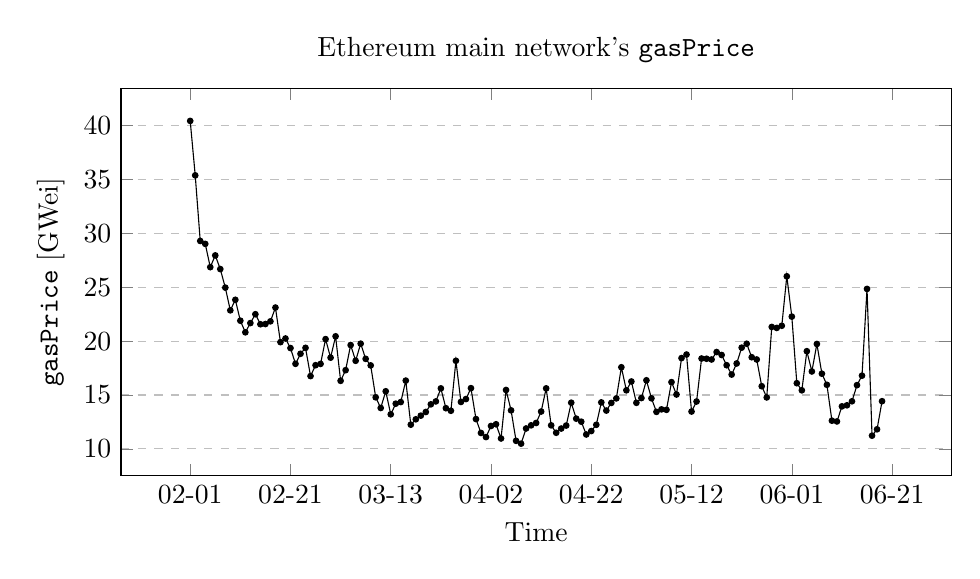
\begin{tikzpicture}
        \begin{axis} [
            title={Ethereum main network's \code{gasPrice}},
            xlabel={Time}, ylabel={\code{gasPrice} [GWei]},
            ytick={10, 15, 20, 25, 30, 35, 40}, 
            ymajorgrids=true, grid style=dashed,
            date coordinates in=x, date ZERO=2018-02-01,
            xticklabel=\month-\day, width=\textwidth, height=6.5cm
        ]

        \addplot[mark=*, mark size=1pt] coordinates {
            (2018-02-01, 40.44) (2018-02-02, 35.39) (2018-02-03, 29.30) (2018-02-04, 29.03) (2018-02-05, 26.87) (2018-02-06, 27.96) (2018-02-07, 26.69) (2018-02-08, 24.97) (2018-02-09, 22.86) (2018-02-10, 23.84) (2018-02-11, 21.90) (2018-02-12, 20.82) (2018-02-13, 21.68) (2018-02-14, 22.50) (2018-02-15, 21.57) (2018-02-16, 21.59) (2018-02-17, 21.84) (2018-02-18, 23.12) (2018-02-19, 19.91) (2018-02-20, 20.25) (2018-02-21, 19.36) (2018-02-22, 17.90) (2018-02-23, 18.83) (2018-02-24, 19.38) (2018-02-25, 16.76) (2018-02-26, 17.77) (2018-02-27, 17.89) (2018-02-28, 20.19) (2018-03-01, 18.47) (2018-03-02, 20.45) (2018-03-03, 16.32) (2018-03-04, 17.31) (2018-03-05, 19.64) (2018-03-06, 18.18) (2018-03-07, 19.77) (2018-03-08, 18.36) (2018-03-09, 17.75) (2018-03-10, 14.79) (2018-03-11, 13.80) (2018-03-12, 15.35) (2018-03-13, 13.21) (2018-03-14, 14.20) (2018-03-15, 14.35) (2018-03-16, 16.34) (2018-03-17, 12.25) (2018-03-18, 12.75) (2018-03-19, 13.09) (2018-03-20, 13.43) (2018-03-21, 14.14) (2018-03-22, 14.41) (2018-03-23, 15.62) (2018-03-24, 13.78) (2018-03-25, 13.54) (2018-03-26, 18.18) (2018-03-27, 14.36) (2018-03-28, 14.63) (2018-03-29, 15.64) (2018-03-30, 12.77) (2018-03-31, 11.48) (2018-04-01, 11.10) (2018-04-02, 12.13) (2018-04-03, 12.29) (2018-04-04, 10.97) (2018-04-05, 15.47) (2018-04-06, 13.58) (2018-04-07, 10.75) (2018-04-08, 10.49) (2018-04-09, 11.90) (2018-04-10, 12.19) (2018-04-11, 12.41) (2018-04-12, 13.47) (2018-04-13, 15.62) (2018-04-14, 12.19) (2018-04-15, 11.50) (2018-04-16, 11.89) (2018-04-17, 12.17) (2018-04-18, 14.29) (2018-04-19, 12.81) (2018-04-20, 12.53) (2018-04-21, 11.34) (2018-04-22, 11.66) (2018-04-23, 12.24) (2018-04-24, 14.32) (2018-04-25, 13.56) (2018-04-26, 14.27) (2018-04-27, 14.69) (2018-04-28, 17.58) (2018-04-29, 15.44) (2018-04-30, 16.26) (2018-05-01, 14.28) (2018-05-02, 14.72) (2018-05-03, 16.37) (2018-05-04, 14.70) (2018-05-05, 13.44) (2018-05-06, 13.67) (2018-05-07, 13.63) (2018-05-08, 16.20) (2018-05-09, 15.05) (2018-05-10, 18.43) (2018-05-11, 18.76) (2018-05-12, 13.47) (2018-05-13, 14.40) (2018-05-14, 18.39) (2018-05-15, 18.37) (2018-05-16, 18.30) (2018-05-17, 18.99) (2018-05-18, 18.72) (2018-05-19, 17.77) (2018-05-20, 16.90) (2018-05-21, 17.93) (2018-05-22, 19.40) (2018-05-23, 19.76) (2018-05-24, 18.51) (2018-05-25, 18.30) (2018-05-26, 15.82) (2018-05-27, 14.78) (2018-05-28, 21.32) (2018-05-29, 21.23) (2018-05-30, 21.43) (2018-05-31, 26.02) (2018-06-01, 22.28) (2018-06-02, 16.10) (2018-06-03, 15.44) (2018-06-04, 19.07) (2018-06-05, 17.19) (2018-06-06, 19.74) (2018-06-07, 16.98) (2018-06-08, 15.95) (2018-06-09, 12.62) (2018-06-10, 12.55) (2018-06-11, 13.95) (2018-06-12, 14.05) (2018-06-13, 14.42) (2018-06-14, 15.92) (2018-06-15, 16.80) (2018-06-16, 24.85) (2018-06-17, 11.23) (2018-06-18, 11.82) (2018-06-19, 14.43)
        };

        \end{axis}
    \end{tikzpicture}
    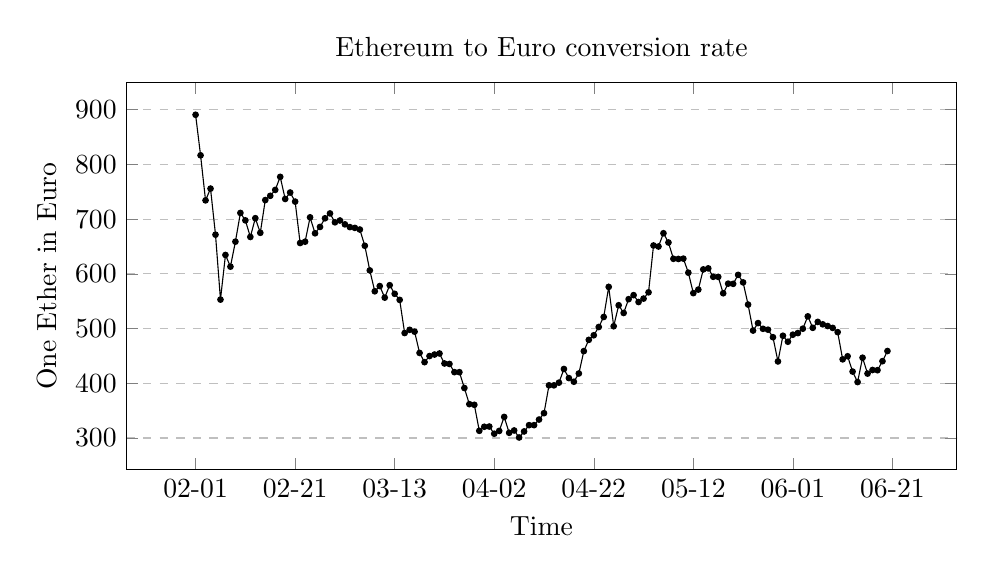
\begin{tikzpicture}
        \begin{axis} [
            title={Ethereum to Euro conversion rate},
            xlabel={Time},
            ylabel={One Ether in Euro},
            ytick={200,300,400,500,600,700,800,900}, 
            ymajorgrids=true, grid style=dashed,
            date coordinates in=x, date ZERO=2018-02-01,
            xticklabel=\month-\day,
            width=\textwidth, height=6.5cm
        ]

        \addplot[mark=*, mark size=1pt] coordinates {
            (2018-02-01, 890.59) (2018-02-02, 816.50) (2018-02-03, 734.20) (2018-02-04, 755.71) (2018-02-05, 671.54) (2018-02-06, 552.93) (2018-02-07, 634.48) (2018-02-08, 613.14) (2018-02-09, 658.79) (2018-02-10, 711.23) (2018-02-11, 697.69) (2018-02-12, 667.37) (2018-02-13, 701.62) (2018-02-14, 674.97) (2018-02-15, 734.74) (2018-02-16, 742.54) (2018-02-17, 753.32) (2018-02-18, 777.17) (2018-02-19, 736.76) (2018-02-20, 748.53) (2018-02-21, 731.95) (2018-02-22, 656.28) (2018-02-23, 658.69) (2018-02-24, 703.21) (2018-02-25, 674.03) (2018-02-26, 685.70) (2018-02-27, 701.50) (2018-02-28, 710.36) (2018-03-01, 694.10) (2018-03-02, 697.46) (2018-03-03, 690.40) (2018-03-04, 685.36) (2018-03-05, 683.93) (2018-03-06, 680.91) (2018-03-07, 651.24) (2018-03-08, 606.24) (2018-03-09, 568.11) (2018-03-10, 577.61) (2018-03-11, 556.52) (2018-03-12, 579.25) (2018-03-13, 563.53) (2018-03-14, 552.42) (2018-03-15, 491.86) (2018-03-16, 497.71) (2018-03-17, 494.36) (2018-03-18, 455.51) (2018-03-19, 438.64) (2018-03-20, 449.81) (2018-03-21, 452.55) (2018-03-22, 454.50) (2018-03-23, 436.22) (2018-03-24, 435.38) (2018-03-25, 420.42) (2018-03-26, 420.33) (2018-03-27, 391.39) (2018-03-28, 361.95) (2018-03-29, 360.75) (2018-03-30, 313.22) (2018-03-31, 320.63) (2018-04-01, 321.03) (2018-04-02, 307.88) (2018-04-03, 313.03) (2018-04-04, 338.59) (2018-04-05, 309.55) (2018-04-06, 313.88) (2018-04-07, 301.04) (2018-04-08, 312.06) (2018-04-09, 323.57) (2018-04-10, 323.60) (2018-04-11, 333.79) (2018-04-12, 345.44) (2018-04-13, 396.31) (2018-04-14, 396.28) (2018-04-15, 401.24) (2018-04-16, 426.16) (2018-04-17, 409.52) (2018-04-18, 402.87) (2018-04-19, 417.95) (2018-04-20, 458.83) (2018-04-21, 479.40) (2018-04-22, 487.76) (2018-04-23, 502.88) (2018-04-24, 521.19) (2018-04-25, 576.12) (2018-04-26, 504.25) (2018-04-27, 542.62) (2018-04-28, 528.54) (2018-04-29, 553.74) (2018-04-30, 561.07) (2018-05-01, 548.51) (2018-05-02, 554.78) (2018-05-03, 566.20) (2018-05-04, 651.81) (2018-05-05, 649.91) (2018-05-06, 674.16) (2018-05-07, 657.24) (2018-05-08, 627.49) (2018-05-09, 627.20) (2018-05-10, 627.76) (2018-05-11, 602.10) (2018-05-12, 564.75) (2018-05-13, 571.19) (2018-05-14, 608.07) (2018-05-15, 609.97) (2018-05-16, 594.58) (2018-05-17, 594.48) (2018-05-18, 564.50) (2018-05-19, 582.05) (2018-05-20, 581.69) (2018-05-21, 598.12) (2018-05-22, 584.35) (2018-05-23, 543.83) (2018-05-24, 496.36) (2018-05-25, 509.99) (2018-05-26, 499.53) (2018-05-27, 497.99) (2018-05-28, 484.20) (2018-05-29, 439.93) (2018-05-30, 486.89) (2018-05-31, 475.98) (2018-06-01, 488.83) (2018-06-02, 491.78) (2018-06-03, 499.79) (2018-06-04, 522.29) (2018-06-05, 501.38) (2018-06-06, 512.19) (2018-06-07, 507.78) (2018-06-08, 504.63) (2018-06-09, 501.25) (2018-06-10, 493.50) (2018-06-11, 443.76) (2018-06-12, 449.39) (2018-06-13, 421.42) (2018-06-14, 402.28) (2018-06-15, 446.75) (2018-06-16, 417.75) (2018-06-17, 424.32) (2018-06-18, 423.95) (2018-06-19, 440.41) (2018-06-20, 458.97)
        };

        \end{axis}
    \end{tikzpicture}

    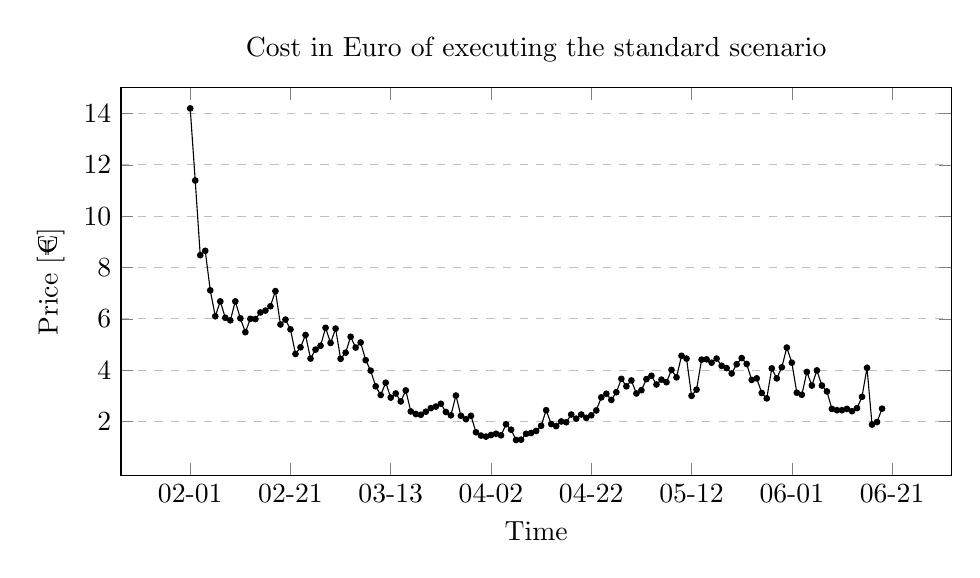
\begin{tikzpicture}
        \begin{axis} [
            title={Cost in Euro of executing the standard scenario},
            xlabel={Time}, ylabel={Price [€]},
            ytick={2, 4, 6, 8, 10, 12, 14}, 
            ymax=15,
            ymajorgrids=true, grid style=dashed,
            date coordinates in=x, date ZERO=2018-02-01,
            xticklabel=\month-\day,
            width=\textwidth, height=6.5cm
        ]

        \addplot[mark=*, mark size=1pt] coordinates {
            (2018-02-01, 14.20) (2018-02-02, 11.39) (2018-02-03, 8.48) (2018-02-04, 8.65) (2018-02-05, 7.11) (2018-02-06, 6.10) (2018-02-07, 6.68) (2018-02-08, 6.04) (2018-02-09, 5.94) (2018-02-10, 6.68) (2018-02-11, 6.02) (2018-02-12, 5.48) (2018-02-13, 6.00) (2018-02-14, 5.99) (2018-02-15, 6.25) (2018-02-16, 6.32) (2018-02-17, 6.49) (2018-02-18, 7.08) (2018-02-19, 5.78) (2018-02-20, 5.97) (2018-02-21, 5.59) (2018-02-22, 4.63) (2018-02-23, 4.89) (2018-02-24, 5.37) (2018-02-25, 4.45) (2018-02-26, 4.80) (2018-02-27, 4.95) (2018-02-28, 5.65) (2018-03-01, 5.06) (2018-03-02, 5.62) (2018-03-03, 4.44) (2018-03-04, 4.68) (2018-03-05, 5.30) (2018-03-06, 4.88) (2018-03-07, 5.08) (2018-03-08, 4.39) (2018-03-09, 3.98) (2018-03-10, 3.37) (2018-03-11, 3.03) (2018-03-12, 3.51) (2018-03-13, 2.93) (2018-03-14, 3.09) (2018-03-15, 2.78) (2018-03-16, 3.21) (2018-03-17, 2.39) (2018-03-18, 2.29) (2018-03-19, 2.26) (2018-03-20, 2.38) (2018-03-21, 2.52) (2018-03-22, 2.58) (2018-03-23, 2.69) (2018-03-24, 2.37) (2018-03-25, 2.24) (2018-03-26, 3.01) (2018-03-27, 2.22) (2018-03-28, 2.09) (2018-03-29, 2.22) (2018-03-30, 1.58) (2018-03-31, 1.45) (2018-04-01, 1.41) (2018-04-02, 1.47) (2018-04-03, 1.52) (2018-04-04, 1.46) (2018-04-05, 1.89) (2018-04-06, 1.68) (2018-04-07, 1.28) (2018-04-08, 1.29) (2018-04-09, 1.52) (2018-04-10, 1.55) (2018-04-11, 1.63) (2018-04-12, 1.83) (2018-04-13, 2.44) (2018-04-14, 1.90) (2018-04-15, 1.82) (2018-04-16, 2.00) (2018-04-17, 1.97) (2018-04-18, 2.27) (2018-04-19, 2.11) (2018-04-20, 2.27) (2018-04-21, 2.14) (2018-04-22, 2.24) (2018-04-23, 2.43) (2018-04-24, 2.94) (2018-04-25, 3.08) (2018-04-26, 2.84) (2018-04-27, 3.14) (2018-04-28, 3.66) (2018-04-29, 3.37) (2018-04-30, 3.60) (2018-05-01, 3.09) (2018-05-02, 3.22) (2018-05-03, 3.65) (2018-05-04, 3.78) (2018-05-05, 3.44) (2018-05-06, 3.63) (2018-05-07, 3.53) (2018-05-08, 4.01) (2018-05-09, 3.72) (2018-05-10, 4.56) (2018-05-11, 4.45) (2018-05-12, 3.00) (2018-05-13, 3.24) (2018-05-14, 4.41) (2018-05-15, 4.42) (2018-05-16, 4.29) (2018-05-17, 4.45) (2018-05-18, 4.17) (2018-05-19, 4.08) (2018-05-20, 3.87) (2018-05-21, 4.23) (2018-05-22, 4.47) (2018-05-23, 4.24) (2018-05-24, 3.62) (2018-05-25, 3.68) (2018-05-26, 3.11) (2018-05-27, 2.90) (2018-05-28, 4.07) (2018-05-29, 3.68) (2018-05-30, 4.11) (2018-05-31, 4.88) (2018-06-01, 4.29) (2018-06-02, 3.12) (2018-06-03, 3.04) (2018-06-04, 3.93) (2018-06-05, 3.40) (2018-06-06, 3.99) (2018-06-07, 3.40) (2018-06-08, 3.17) (2018-06-09, 2.49) (2018-06-10, 2.44) (2018-06-11, 2.44) (2018-06-12, 2.49) (2018-06-13, 2.40) (2018-06-14, 2.52) (2018-06-15, 2.96) (2018-06-16, 4.09) (2018-06-17, 1.88) (2018-06-18, 1.98) (2018-06-19, 2.50)
        };

        \end{axis}
    \end{tikzpicture}
\end{center}
\end{figure}

The last cost that has to be discussed is the contract deployment cost. The deployment scheme we used is the one suggested by the Truffle framework. The first deployment on a chain requires deploying two contracts: the actual smart contract we are interested in and and additional \code{Migrations} contract managed by Truffle that keeps track of which migration scripts have been run on the current chain and which have not. Deploying these two contracts on the Rinkeby test network has some significant costs, as described in table \ref{table:deployment-costs}. This data can be obtained by inspecting the data associated with the following transactions:

\begin{itemize}
    \item \txmigrationsdepoly: deployment \\ of the \code{Migrations} smart contract
    \item \txupdatemiga: update of \\ the last successful migration
    \item \txmaindeploy: deployment \\ of the \code{Main} smart contract
    \item \txupdatemigb: update of \\ the last successful migration
\end{itemize}

\begin{table}[tp]
    \caption[Cost of deploying the smart contract]{Costs of deploying the smart contract. This table assumes a \code{gasPrice} of \gaspricegwei and an exchange rate between Ether and Euro of \ethtoeur}
    \centering
    \label{table:deployment-costs}
    \begin{tabular}{c c c c}
        \toprule
        Contract & Gas consumed [Units] & Ether cost [GWei] & Euro cost [€]\\ 
        \midrule
        Migrations & 319470 & 5434537.14 & 2.92 \\ Main & 3158630 & 53731780.87 & 28.87 \\ Total & 3478100 & 59166318.01 & 31.79 \\
        \bottomrule
    \end{tabular}
\end{table}

From these results, we can see that the development costs for this smart contract are quite high: every update to the application requires deactivating the old contract and deploying a new one, incurring in the associated costs. Proper testing and extensive review before every deployment are therefore necessary in order to avoid any unnecessary deployment costs.

\subsection{Discussion}
As already said, the true solution to the problem encountered while desining this application would be verifiable computing. Unfortunately, the technology is not viable yet and this forced us to take an alternative path. Overall, we think we succeded in our goal of providing a decentralized market for computational power in which the incentives put in place offer some degree of reliablity to the users of the system.

However, some important consideration that emerged from the development of our proof of concept have to be discussed. In particular, the system has some non-negligible costs for the users and these fees are much higher than those offered by common cloud providers: this could significantly slow down the adoption of our solution. An additional concern is the overall slowness of the system: in order to be mined, every transaction takes a minimum of fifteen seconds (the mining time of a block) and this could pose some severe limitions on the scale at which this system could be employed.

A final point that should be considered is the difficulty of updating the smart contract (that is, deactivating the old one and deploying a new one). The costs involved make this process very onerous and limit the number of updates that can be released. Another aspect of this update procedure, that makes it even more difficult, is that all the users of the service must be notified of the address of the new contract: this is notoriously difficult in a decentralized environment like the blockchain one.

%!TEX root = ../thesis.tex

\section{Conclusion and future work}
\label{sect:conclusions-and-future-work}

\subsection{Smart contract}
The smart contract implementation that we developed takes into consideration most of the use cases described in section \ref{sect:requirements}. However, there are still some aspects that should be improved.  
In particular, in the current version, the handling of the ownership of the contract and of whom can perform auditing duties is very limited. The current system could be improved by having more than a single trusted member and by requiring some kind of voting procedure before changing the contracts' configuration parameters. Another enhancement would be to better distribute the auditing duties, instead of forcing the contract's owner to be the only auditor.  

Another situation in which some improvements are required is the result's submission methodology, which, as of now, is again very limited: for example, the publisher could specify a public key with which the results should be encrypted before being uploaded.
A final enhancement would be to provide an administrative method that allows to perform some garbage collection: as of now, all the metadata regarding past computations (e.g. Docker image name, publisher address, ...) are stored on chain. There should be a way for someone with administrative rights to trigger a cleanup that removes all computations that cannot change state anymore.

\subsection{Client application}
The client application is really bare-bone and has been developed only to have a practical way of interacting with the smart contract.  Further versions of this application could be improved in several way and would probably require a complete redesing of the user interface.
Additionally, this client application should become more automatic: in the current version, many actions are manual. In particular, accepting to perform a published computation is a manual step which could be automated: the farmer should simply specify some contraints (e.g. on the reward or the stake fee) and then the application should automatically try to accept the computation that satisfy these contraints. Another improvement could be to automatically download the results of a computation when they are accepted and check that the hash of the downloaded archive matches the one reported by the farmer.

An additional enhancement could be to only consider Docker image names that contain the image digest and automatically discard all published computations that rely on image tags instead.
A final improvement that should be done is to embedd auditing functionalities in the application: as of now, the client application is not able to act as an auditor.




% ********************************** Back Matter *******************************
% Backmatter should be commented out, if you are using appendices after References
%\backmatter

% ********************************** Bibliography ******************************
\begin{spacing}{0.9}

% To use the conventional natbib style referencing
% Bibliography style previews: http://nodonn.tipido.net/bibstyle.php
% Reference styles: http://sites.stat.psu.edu/~surajit/present/bib.htm

\bibliographystyle{apalike}
%\bibliographystyle{unsrt} % Use for unsorted references  
%\bibliographystyle{plainnat} % use this to have URLs listed in References
\cleardoublepage
\bibliography{References/references} % Path to your References.bib file


% If you would like to use BibLaTeX for your references, pass `custombib' as
% an option in the document class. The location of 'reference.bib' should be
% specified in the preamble.tex file in the custombib section.
% Comment out the lines related to natbib above and uncomment the following line.

%\printbibliography[heading=bibintoc, title={References}]


\end{spacing}

% ********************************** Appendices ********************************

%\begin{appendices} % Using appendices environment for more functunality
%
%\include{Appendix1/appendix1}
%\include{Appendix2/appendix2}
%
%\end{appendices}

% *************************************** Index ********************************
\printthesisindex % If index is present

\end{document}
\grid
